\pdfoutput=1
\documentclass[article,aps,nofootinbib,twocolumn,superscriptaddress]{revtex4-1}
\input epsf
\usepackage{graphics}
\usepackage{amsmath}
\usepackage{amssymb}
\usepackage{bm}
\usepackage{braket}
\usepackage{booktabs}
\usepackage{subfigure}
\usepackage{subfloat}
\usepackage{float}
\usepackage[usenames,svgnames]{xcolor}
\usepackage{hyperref}

\hypersetup{
    colorlinks=true,
    urlcolor=SteelBlue,
    linkcolor=red,
    citecolor=blue,
}


\usepackage{color}
\usepackage{dcolumn}
\usepackage{hyphenat}


\def\be{\begin{equation}}
\def\ee{\end{equation}}
\def\ba{\begin{eqnarray}}
\def\ea{\end{eqnarray}}

\newcommand{\ack}[1]{[{\bf Pfft!#1}]}
\newcommand{\tvb}[1]{{\bf \color{blue}{{#1}}}}
\newcommand{\tvg}[1]{{\bf \color{green}{{#1}}}}
\newcommand{\tvr}[1]{{\bf \color{red}{{#1}}}}
\newcommand{\ay}[1]{{\bf \color{magenta}{{#1}}}}

%\maketitle
\usepackage{graphicx}

\begin{document}

\title{Echoes from the scattering of wavepackets on wormholes}

\author{Jos\'e T. G\'alvez Ghersi}
\email{joseg@sfu.ca}
\author{Andrei V. Frolov}
\email{frolov@sfu.ca}
\author{David Dobre}
\email{ddobre@sfu.ca}
\affiliation{Department of Physics, Simon Fraser University, Burnaby, BC, V5A 1S6, Canada}


\begin{abstract}
In the light of the recent progress showing that the hypothetical observation of pulses isolated from the gravitational radiation transient (also known as echoes) would prove the existence of exotic compact objects (ECOs); it is possible to reproduce many features of the ringdown signal by simulating a scattering problem instead of the full coalescence of ECOs. In this paper, we study the dynamics of scalar and tensor wavepackets colliding against a spherically symmetric traversable wormhole. Our purpose is to extract the features of the time-dependent scattering solutions inside and outside the effective potential cavity in addition to their asymptotic behavior. Using the geometrical optics approximation, we show that the amplitude of the echoes is only large enough in a narrow bandwidth of frequency space, where the intensity of the transient reduces. The computer code used to produce these results is publicly available for further applications, including scattering and accretion processes.      
\end{abstract}

\maketitle


\section{Introduction}
The era of gravitational wave (GW) astronomy \citep{Abbott:2016blz, Abbott:2016nmj} has begun. GW spectroscopy, in contrast to its atomic counterpart, allows us to characterize strong gravitational interactions in their radiative regime. In this new range of frequencies, it is now possible to explore the role of dynamical gravitational degrees of freedom in a wide range of astrophysical \citep{Frolov:2017asg, Cardoso:2016rao} and cosmological \citep{Krauss989, Ade:2018gkx} phenomena. 

The prolonged absence of observational evidence confirming the dynamical properties of spacetime has motivated a plethora of conjectures about the behaviour of gravity within and beyond \citep{Clifton:2011jh, Taliotis:2012sx, Joyce:2014kja} classical General Relativity (GR). Latterly, the potential existence of exotic compact objects (ECOs) sourced by quantum effects on gravity \citep{PhysRevLett.61.1446, Almheiri:2012rt, Mazur:2001fv} (such as wormholes, firewalls and gravastars) has captured the attention of many recent efforts \citep{Cardoso:2016oxy, Abedi:2016hgu, Abedi:2018npz}. Wherein the primary claim is that the detection of a train of ``echoes'' isolated from the main transient of GW and with generically large amplitudes would be clear evidence of ECOs. It is, therefore, necessary to understand (i) the mechanisms behind the production of echoes and (ii) the intensity and spectrum of the outgoing wavelets compared to the GW transient in the most straightforward possible setup. In this paper, we explore the generation of echoes by colliding wavepackets of scalar and tensor radiation against a traversable spherically symmetric wormhole \citep{Visser:1989kh}. Such a wormhole behaves just like a Fabry-Perot cavity, shares common properties with the effective potential cavities made by other ECOs, like gravastars and firewalls, and the main features of the dispersed pulses are similar to the ringdown signals after the coalescence of ECOs.

Here we consider a wormhole configuration made by the junction of two Schwarzschild geometries of equal masses at $r_0>2M$, just as shown in \citep{Cardoso:2016oxy}. In this case, the symmetry of the centrifugal barriers at $r=3M$ on each side of the throat allows us to find the reflection and transmission coefficients of the cavity. Hence, it is possible to reconstruct the spectral shape of the outgoing pulse using the geometrical optics approximation. Nevertheless, this approximation predicts an exponential decay of the subsequent higher order reflections, which appears instead as a power law in the full solution of the scattering problem. Thus, the excitation of quasinormal modes (QNMs) is the only cause for the presence of echoes in the time evolving profile, these modes are sourced by a sequence of internal reflections inside the potential cavity and then propagate throughout the surface of the maximal potential energy spheres (i.e., the ``edges'' of the potential barriers), while leaking energy into the exterior. QNMs of the Schwarzschild solution have been extensively studied and reproduced in various analytic and numerical simulations \citep{Chandrasekhar:1975zza, PhysRevD.46.4179}; thus it is easy to identify their characteristic frequencies in the spectrum of outgoing pulses. We as well present the full scattering solution both inside and outside the wormhole cavity in detail, along with the energy fluxes and the asymptotic solutions for the principal spherical modes of a scalar (and tensor) wavepackets. In addition to this, we find the width and frequency intervals contained in the incident wavepackets for which the outgoing the wavelets have maximal amplitudes. Our computer code is optimized to solve both scalar accretion and scattering problems and is publicly available in \url{https://github.com/andrei-v-frolov/accretion/tree/wormhole}.

The layout for this paper is as follows: in section \ref{sec:scalar}, we review the scattering problem of scalar waves starting by a quick overview of the dispersion of a Gaussian pulse by a Schwarzschild black hole. In this review, we will be able to calculate the transmission and reflection coefficients of the centrifugal barriers constituting the walls of the resonant cavity in the case of the wormhole. Our results show a frequency ``sweet spot'' such that the incident pulse is not fully reflected nor fully transmitted by the cavity, favouring multiple internal reflections that source the QNMs.  Furthermore, we solve the scattering problem by a wormhole directly using the same ingoing Gaussian wavepacket, and then we compare the Fourier transform of this solution with the pulse reconstructed following the geometrical optics approximation. We find that the approximate reconstruction matches the full solution, up to the peaks due to the QNM frequencies. Likewise, we evaluate the amplitude of each of the echoes as a function of the width of the initial gaussian waveform, finding that a single width of the incident pulse maximizes the amplitude of each echo. In section \ref{sec:tensor}, we extend all the results in the previous section for a Gaussian pulse of tensor fluctuations of the metric by following the even and odd decomposition of the tensor modes introduced by Regge, Wheeler and Zerilli in \citep{Regge:1957td, PhysRevD.2.2141, PhysRevD.5.2419, PhysRevD.5.2439}. Our results can be recasted in terms of the usual asymptotic polarization modes $h_+$ and $h_{\times}$, known as the perturbations of a flat metric. Finally, in section \ref{sec:conclusions}, we discuss and conclude.

\section{Scattering of scalar wavepackets}\label{sec:scalar}
In this section, we solve the scattering of a Gaussian wavepacket by a spherically symmetric wormhole. To do so, we will first review the dispersion by the centrifugal barrier of a spherically symmetric black hole in order to find the properties of the potential cavity.
\subsection{Scattering by a Schwarzschild black hole}
The dispersion of scalar waves by a Schwarzschild black hole has been thoroughly studied \citep{doi:10.1063/1.522949, Sanchez:1976xm, Sanchez:1977si, Sanchez:1977vz}, it is crucial for our purposes to provide the full solution since it contains all the information of the potential barriers constituting the effective potential in the case of a wormhole. The dynamics of the scattering problem is found by solving the equation of motion for scalar field
\begin{equation}
\Box\Phi=0,\label{eq:scalar_eq_mov} 
\end{equation}
where $\Box\equiv g^{\alpha\beta}\nabla_{\alpha}\nabla_{\beta}$ is the standard d'Alembertian in a curved background. Here $g_{\alpha\beta}$ is the metric tensor in a spherically symmetric Schwarzschild-like static spacetime
\begin{equation}
g_{\alpha\beta}=-f(r)\delta^t_{\alpha}\delta^t_{\beta}+\frac{1}{f(r)}\delta^r_{\alpha}\delta^r_{\beta}+r^2\left(\delta^{\theta}_{\alpha}\delta^{\theta}_{\beta}+\sin^2\theta\delta^{\phi}_{\alpha}\delta^{\phi}_{\beta}\right).
\label{eq:Schwarzschild}
\end{equation}
\begin{figure}[t]
\centering
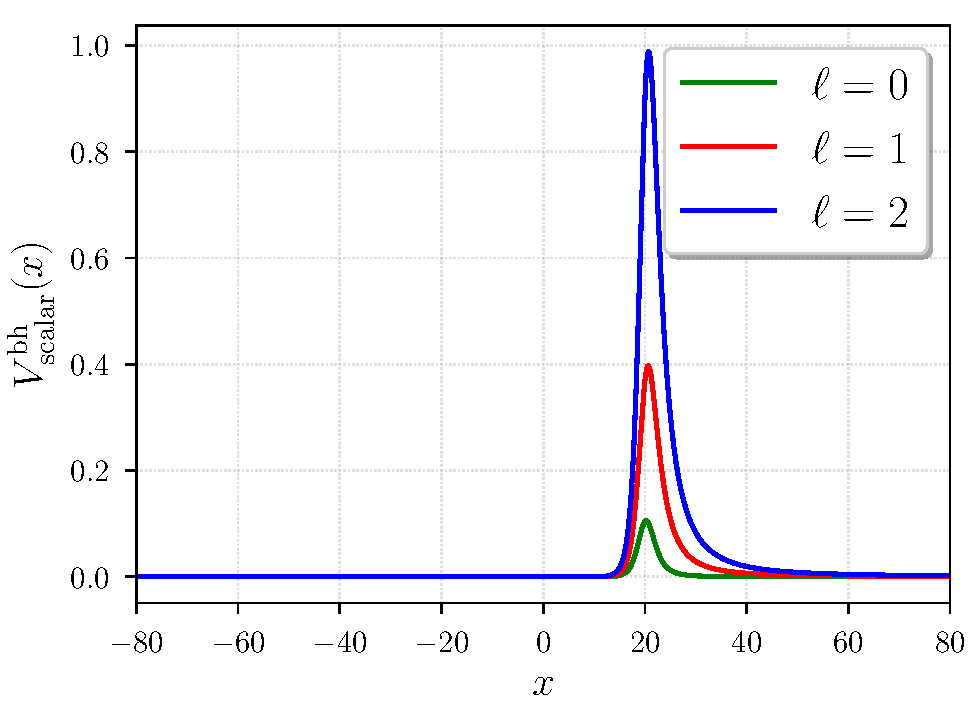
\includegraphics[width=.45\textwidth]{figures/potential_scalar_bh.pdf}
\caption{\label{fig:Potential_BH} Effective potential for the spherical modes $\mathcal{U}_{\ell m}(x,t)$ scattered by a Schwarzschild black hole, growing with $\ell$. The wall acts as a barrier transparent to certain frequencies above a transmissivity threshold and reflective for lower frequencies.}
\end{figure}
It is convenient to introduce the tortoise coordinate $x$:
\begin{equation}
x\equiv\displaystyle{\int_{r_0}^r\frac{dr}{f(r)}},
\label{eq:tortoise}
\end{equation} 
In the case of the Schwarzschild metric $f(r)=1-r_g/r$ the last expression yields
\begin{equation}
x=r-r_0+r_g\ln\left(\frac{r-r_g}{r_0-r_g}\right),
\label{eq:tortoise2}
\end{equation} 
for $r_g<r<+\infty$ and $r_0>r_g$, where $r_g=2M$ is the usual Schwarzschild radius. By direct evaluation, we see that $r=r_0$ corresponds to $x=0$, the horizon $r=2M$ maps into $x\rightarrow-\infty$ and $r\rightarrow+\infty$ is $x\rightarrow+\infty$. In our numerical routine, we invert \eqref{eq:tortoise2} to get $r\equiv r(x)$ (see the appendix A, subsection 6 in \citep{Frolov:2017asg} for more details). In tortoise coordinates, we can decompose the scalar field in spherical harmonics 
\begin{equation}
\Phi(x,t)=\frac{1}{r(x)}\sum_{\ell,m=0}\mathcal{U}_{\ell m}(x,t)Y_{\ell m}(\theta,\phi),
\label{eq:ylm_decomp}
\end{equation}
in that way we can rewrite \eqref{eq:scalar_eq_mov} as
\begin{equation}
\left[-\partial_t^2+\partial_x^2-V_{\mathrm{scalar}}(x)\right]\mathcal{U}_{\ell m}(x,t) = 0,
\label{eq:wave_scalar}
\end{equation}
and the effective potential $V_{\mathrm{scalar}}(x)$ is given by
\begin{equation}
V_{\mathrm{scalar}}(x) = \left(1-\frac{r_g}{r(x)}\right)\left[\frac{\ell(\ell+1)}{r(x)^2}+\frac{r_g}{r(x)^3}\right].
\end{equation}
After rearranging the variables, the equation of motion of the spherical modes is now written in its traditional linear waveform. In Fig.~\ref{fig:Potential_BH}, we observe the growth of the potential barrier with the quantum number $\ell$. The potential wall does not vanish for the monopole ($\ell=0$) due to the extra term proportional to $r^{-3}$ appearing after the coordinate change, which replaces the radial damping in the original Schwarzschild coordinates $(t,r)$. Such a term becomes subdominant for all $\ell\geq 1$. Intuitively, it is reasonable to expect that the modes with frequency above a given threshold can cross the barrier, while reflecting the lower frequency modes. 

Now we setup the scattering problem for one of the spherical modes ($\mathcal{U}_{20}$, the quadrupole) with the following initial conditions corresponding to an ingoing Gaussian wavepacket 
\begin{equation}
\mathcal{U}_{20}(x,0)=\exp\left(\frac{(x-x_0)^2}{2\sigma^2}\right)~,~\frac{d \mathcal{U}_{20}}{dt}\bigg{|}_{t=0}=\frac{d \mathcal{U}_{20}(x,0)}{dx},
\label{eq:scalar_init_cond}
\end{equation}

\begin{figure}[t!]
\centering
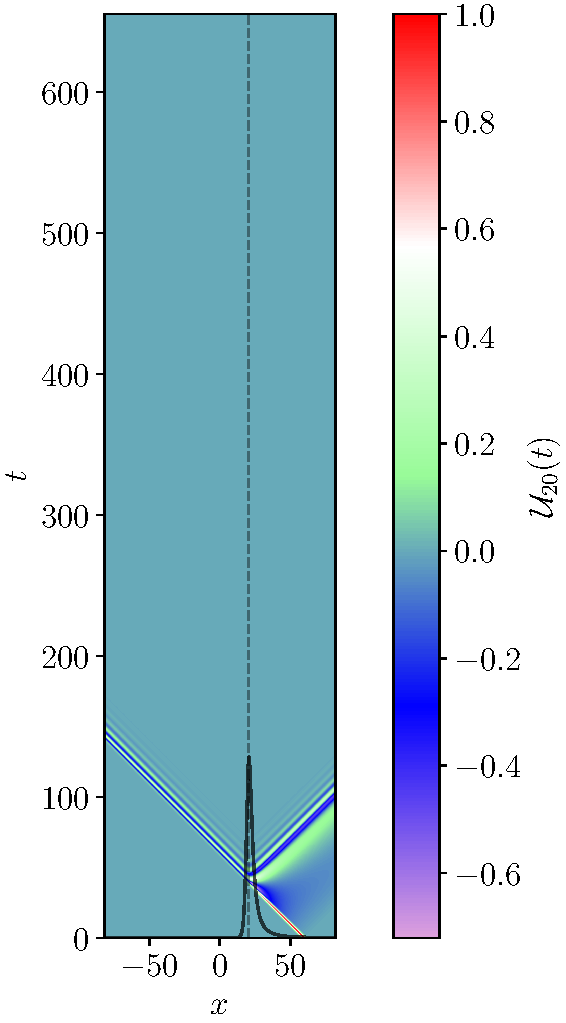
\includegraphics[width=.45\textwidth]{figures/bh_l_2.pdf}
\caption{\label{fig:bh_sol} Dispersion of the ingoing Gaussian wavepacket $\mathcal{U}_{20}$ by the potential barrier (plotted in black) showing the incident, reflected and transmitted pulses, it is possible notice the ringing of the reflected solution due to the quasinormal modes.}
\end{figure}

\begin{figure}[t]
\centering
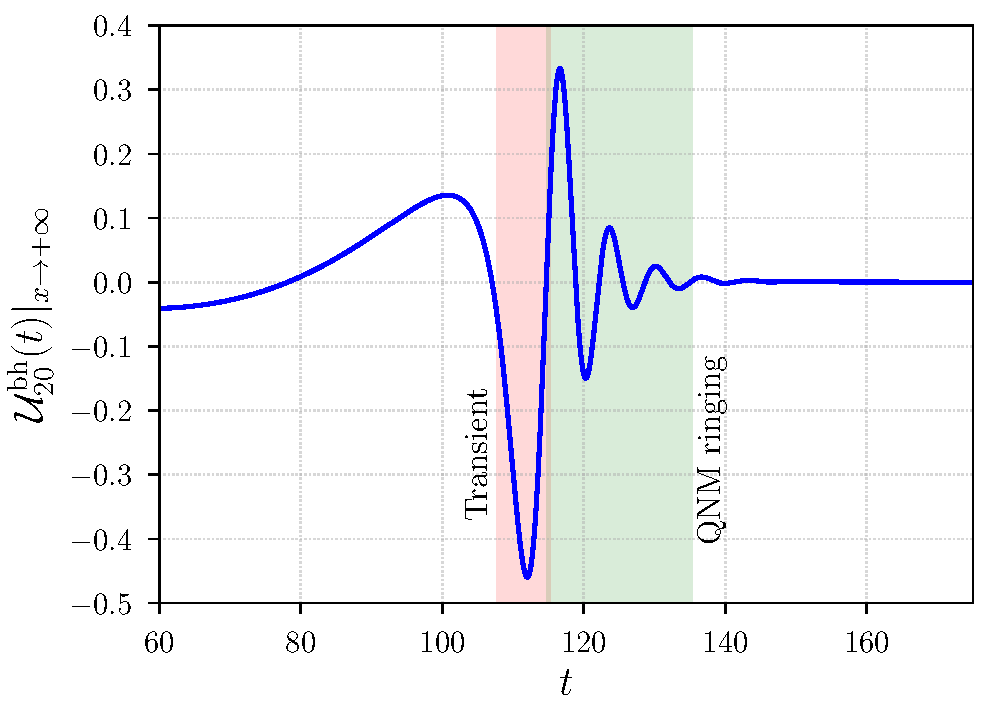
\includegraphics[width=.45\textwidth]{figures/Scalar_bh.pdf}
\caption{\label{fig:asympt_sol} Asymptotic solution for the quadrupole mode $\mathcal{U}_{20}(x,t)$ by direct evaluation of the results in Fig.~\ref{fig:bh_sol}. The reflected signal shows its maximum peak and the posterior ringing due to QNMs.}
\end{figure}

\begin{figure}[t]
\centering
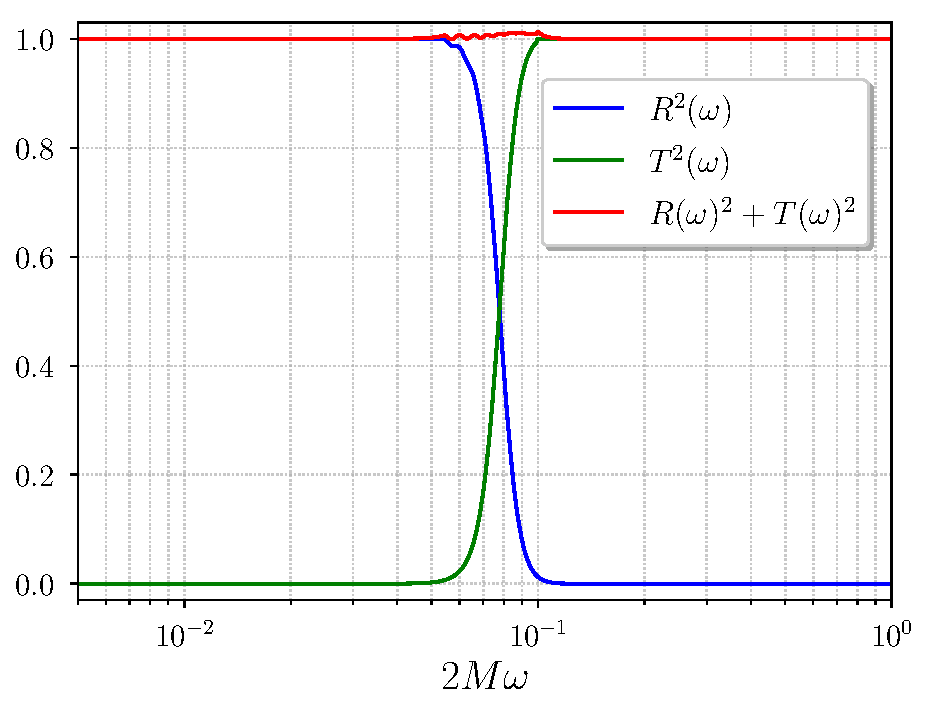
\includegraphics[width=.45\textwidth]{figures/RT_omega_scalar.pdf}
\caption{\label{fig:RT_scalar} Reflection and transmission coefficients as a function of frequency $(\omega)$, the identity $R^2+T^2=1$ is fulfilled with an error smaller than 1\%.}
\end{figure}

After fixing the values of the width to be $\sigma=2.598r_g$, the initial position of the Gaussian at $x_0=60.0r_g$, $r_0=20.0r_g$ and the initial conditions in \eqref{eq:scalar_init_cond}, we show the time-dependent solution of \eqref{eq:wave_scalar} in Fig.~\ref{fig:bh_sol}, where we distinguish the incident, transmitted and reflected parts of the solution. It is important to observe the absence of spurious late time reflections and interferences due to the implementation of perfectly matching layers (PMLs) in the outermost regions of our simulation box (see the details of our setup for PMLs in \citep{Frolov:2017asg}). We observe the main features of the reflected signal in Fig.~\ref{fig:asympt_sol}, where the asymptotic behavior of the signal shows a sharp transient is a consequence of the collision against the potential wall, and the ringing of quasinormal modes occuring right after the reflection in agreement with \citep{Petrich:1985csm}. 

It is now possible to evaluate the reflection and transmission coefficients of the potential wall depicted in Fig.~\ref{fig:Potential_BH}. To do so, we compute the one dimensional Fourier transform of the incident $\tilde{\mathcal{U}}_{20}^{\mathrm{inc}}(\omega)=\mathcal{F}[\mathcal{U}_{20}(0,x)]$, reflected $\tilde{\mathcal{U}}_{20}^{\mathrm{ref}}(\omega)=\mathcal{F}[\mathcal{U}_{20}(t,+\infty)]$ and transmitted $\tilde{\mathcal{U}}_{20}^{\mathrm{trans}}(\omega)=\mathcal{F}[\mathcal{U}_{20}(t,-\infty)]$ from the solved scattering modes in order to define
\begin{equation}
R(\omega)\equiv \frac{||\tilde{\mathcal{U}}_{20}^{\mathrm{ref}}(\omega)||}{||\tilde{\mathcal{U}}_{20}^{\mathrm{inc}}(\omega)||}~,~T(\omega)\equiv \frac{||\tilde{\mathcal{U}}_{20}^{\mathrm{trans}}(\omega)||}{||\tilde{\mathcal{U}}_{20}^{\mathrm{inc}}(\omega)||}
\label{eq:ref_and_trans}
\end{equation}
as the transmission and reflection coefficients, respectively. In Fig.~\ref{fig:RT_scalar}, we plot the squares of these coefficients as functions of frequency observing that the identity $R^2+T^2=1$ is only approximately met because of the small contributions coming from the QNMs frequency peaks in both the transmitted and reflected solutions. The shape of both the transmissivity and reflectivity curves is very similar to an hyperbolic tangent step function\footnote{This is not surprising after we consider the DeWitt approximation for the transmissivity \citep{Frolov:1998wf}, which is precisely given by a step function.}, intersecting at $R^2=T^2=0.5$, as expected. Furthermore, it is crucial to notice from the last figure that it is only in a narrow band of frequencies where the amplitudes transmitted and reflected by the potential barrier are comparable. Such a fact will be important in our analysis of the effective potential cavity in the case of a wormhole.  
\subsection{Scattering by a traversable wormhole} 



\section{Scattering of tensor wavepackets}\label{sec:tensor} 
\section{Conclusions}\label{sec:conclusions}

\bibliography{bibliography.bib}

\end{document}
